\documentclass[hyperref={pdfpagemode=FullScreen}, aspectratio=169, 10pt]{beamer}

\usetheme[progressbar=frametitle]{metropolis}
\usepackage{appendixnumberbeamer}

\usepackage{booktabs}
\usepackage[scale=2]{ccicons}

\usepackage{pgfplots}
\usepgfplotslibrary{dateplot}

\usepackage{xspace}
\newcommand{\themename}{\textbf{\textsc{metropolis}}\xspace}

% pifont has dingbats and funny symbols
\usepackage{pifont}
\newcommand{\cmark}{\ding{51}}%
\newcommand{\xmark}{\ding{55}}%

% Tikz stuff
\usepackage{tikz}
\usepackage{tikzpeople}

% graphics
\usepackage{graphicx}
\graphicspath{ {assets/} }

% plotting stuff
\usepackage{pgfplots}
\pgfplotsset{compat=1.18}
\usetikzlibrary{intersections,decorations.markings}

\newcommand{\plotcurve}[3][thick, every plot/.style={smooth}]{
  % plot curve y^2 = x^3 + a x + b in range [-3,3]^2
  % parameter 1 (optional): style options for curve (color, etc)
  % parameter 2: curve parameter a
  % parameter 3: curve parameter b
  \draw[gray] (-3,-3) rectangle (3,3);
  \draw[->,>=latex,gray] (-3,0) -- (3,0);
  \draw[->,>=latex,gray] (0,-3) -- (0,3);
  \draw[name path=curve, #1] plot[id=curve#2#3, raw gnuplot] function {
    f(x,y) = y**2 - x**3 - #2*x - #3;
    set xrange [-3:3];
    set yrange [-3:3];
    set view 0,0;
    set isosample 50,50;
    set cont base;
    set cntrparam levels incre 0,0.1,0;
    unset surface;
    splot f(x,y);
  };
}

\tikzset{
  tangent/.style={
    decoration={markings, mark=at position #1 with {
      \coordinate (tangent point-\pgfkeysvalueof{/pgf/decoration/mark info/sequence number}) at (0pt,0pt);
      \coordinate (tangent unit vector-\pgfkeysvalueof{/pgf/decoration/mark info/sequence number}) at (1,0pt);
      \coordinate (tangent orthogonal unit vector-\pgfkeysvalueof{/pgf/decoration/mark info/sequence number}) at (0pt,1);
    }},
    postaction=decorate
  },
  use tangent/.style={
    shift=(tangent point-#1),
    x=(tangent unit vector-#1),
    y=(tangent orthogonal unit vector-#1)
  },
  use tangent/.default=1
}

\title{Exploring Password Authenticated Key Exchange Algorithms}
\subtitle{Final Year Project Screencast}
\author{Sam Leonard}
\institute{Supervisor: Bernardo Magri}
\date{}

\begin{document}

\maketitle

% talk about what you are going to talk about, state you will explain PAKEs
\begin{frame}{Table of contents}
  \setbeamertemplate{section in toc}[sections numbered]
  \tableofcontents%[hideallsubsections]
\end{frame}

\section[Intro]{Introduction}

% talk about how auth is broke
\begin{frame}{Motivation}
  \begin{figure}[H]
    \centering
    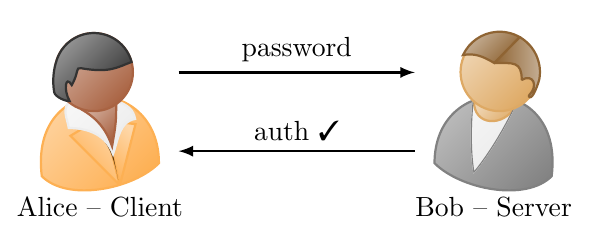
\begin{tikzpicture}[thick,>=latex]
      \node[alice,minimum size=1.5cm] at (0,0) {Alice -- Client};
      \node[bob,mirrored,minimum size=1.5cm] at (5,0) {Bob -- Server};
      \draw[->] (1,0.5) -- (4,0.5) node[midway, above] {password};
      \draw[->] (4,-0.5) -- (1,0-0.5) node[midway, above] {auth \cmark};
    \end{tikzpicture}
  \end{figure}
\end{frame}

% talk about how PAKEs are different, state that this is a balanced PAKE
% mention augmented pakes where password is replaced with a verifier
\begin{frame}{Motivation}
  PAKEs are a radically different solution to this problem.
\end{frame}

% talk about how implemented AuCPace in Rust and open sourced the implementation through RustCrypto
\begin{frame}{Project Summary}
  I made an awesome PAKE in Rust
\end{frame}

\section{Context}

\begin{frame}{What are PAKEs?}
  \begin{figure}[H]
    \centering
    \begin{tikzpicture}[thick,>=latex]
      \node[alice,minimum size=1.5cm] at (9,0) {Alice -- Client};
      \node[bob,mirrored,minimum size=1.5cm] at (14,0) {Bob -- Server};
      \node at (10.3,0.8) {password};
      \draw[->] (10, 0.5) -- (10,-0.5) node[midway, right, xshift=0.1cm, yshift=0.1cm, scale=0.05] {
\includegraphics{wand.png}};
      \node[scale=0.02] at (10.3,-0.7) {
\includegraphics{key.png}};
      \node at (12.8,0.8) {password};
      \draw[->] (13, 0.5) -- (13,-0.5) node[midway, left, xshift=-0.1cm, yshift=0.1cm, scale=0.05] {
\includegraphics{wand.png}};
      \node[scale=0.02] at (12.5,-0.7) {
\includegraphics{key.png}};
      \draw[<->] (10.8,-0.7) -- (12,-0.7) node[midway, below] {auth \cmark};
    \end{tikzpicture}
  \end{figure}
\end{frame}

\begin{frame}{Elliptic Curves}
  \begin{center}
  \begin{tikzpicture}[thick,>=latex,scale=0.8]
    \begin{scope}
      \draw[<->,gray] (-3,0) -- (3,0) node[right] {$x \in \mathbb{R}$};
      \draw[<->,gray] (0,-3) -- (0,3) node[above] {$y \in \mathbb{R}$};
      \draw[thick, name path=curve, every plot/.style={smooth}] plot[id=weierstrass-curve-1, raw gnuplot] function {
        f(x,y) = y**2 - (x**3 - 2.5*x + 1);
        set xrange [-3:3];
        set yrange [-3:3];
        set view 0,0;
        set isosample 50,50;
        set cont base;
        set cntrparam levels incre 0,0.1,0;
        unset surface;
        splot f(x,y);
      };
    \end{scope}

    \node at (0,-4) {$y^2 = x^3 - 2 x - 1$ over $\mathbb{R}$};
  \end{tikzpicture}
  \end{center}
\end{frame}

\begin{frame}{Point addition}
  \begin{center}
  \begin{tikzpicture}[scale=.45]
    \begin{scope}[xshift=0cm]
      \plotcurve{-2}{2}
      \draw[->, >=latex, thick] (-2.5,-1) -- ++(0,3.5) node[right] {$\mathcal{O}$};
      \node[below] at (0,-4) {Neutral element $\mathcal{O}$};
    \end{scope}

    \begin{scope}[xshift=7.5cm]
      \plotcurve{-2}{2}
      \draw[dashed, semithick, name path=vertical] (-1.25,2.5) -- ++(0,-5);
      \draw[name intersections={of=curve and vertical}] (intersection-1) node {$\bullet$} node[above left] {$P$}
      (intersection-2) node {$\bullet$} node[below left] {$-P$};
      \node[below] at (0,-4) {Inverse element $-P$};
    \end{scope}

    \begin{scope}[xshift=15cm]
      \plotcurve{-2}{2}
      \draw[thick, name path=chord] (-2.5,.5) -- (2.5,2.0);
      \draw[name intersections={of=curve and chord}] (intersection-1) node {$\bullet$} node[above left] {$P$}
      (intersection-2) node {$\bullet$} node[above right=-1pt] {$Q$}
      (intersection-3) node {$\bullet$} coordinate[name=mPQ];
      \draw[dashed, semithick, name path=vertical] (mPQ) ++(0,1) -- +(0,-5.5);
      \draw[name intersections={of=curve and vertical}] (intersection-2) node {$\bullet$} node[below left] {$P+Q$};
      \node[below, align=center] at (0,-4) {Addition $P+Q$ \\ ``Chord rule''};
    \end{scope}

    \begin{scope}[xshift=22.5cm]
      \plotcurve[thick, tangent=0.265, every plot/.style={sharp plot}]{-2}{2}
      \draw[thick, use tangent, name path=chord] (-.6,0) -- (1.5,0);
      \draw[name intersections={of=curve and chord}] (intersection-1) node {$\bullet$} node[above] {$P$}
      (intersection-2) node {$\bullet$} coordinate[name=mPQ];
      \draw[dashed, semithick, name path=vertical] (mPQ) ++(0,1) -- +(0,-5.0);
      \draw[name intersections={of=curve and vertical}] (intersection-2) node {$\bullet$} node[below left] {$2P$};
      \node[below, align=center] at (0,-4) {Doubling $P+P$ \\ ``Tangent rule''};
    \end{scope}

  \end{tikzpicture}
\end{center}

\end{frame}

\begin{frame}{Finite Fields}
  clock maths
\end{frame}

\begin{frame}{Elliptic Curves Over Finite Fields}
  dotty curves
\end{frame}

\begin{frame}{AuCPace}
  Augmented Composable what now?
\end{frame}

\section{Demo}

\begin{frame}{Conclusion}
  I did a thing!
\end{frame}

\begin{frame}[standout]
  Thank you for watching!
\end{frame}

\end{document}
